\section{Easy Web Content Site builder.}

We call it EWS. The main project we are working on is a new online site builder. This project intend to complete the existing Easy Web Content service.
%descriptopn of EWC
Basically The site builder will make extensive usage of ajax. The main directions of the project are
\begin{itemize}
\item Be the most simple in terms of user experience
\item propose simple to create but adapted styles and easy to customise
\item does not have the drawbacks of the concurrence
\item have the advantages of the concurrence
\item be scalable
\item be securized
\item target users : 2/3 of them have no HTML/CSS knowledge
\end{itemize}

%show a sample of the concurrence

So the first stpe into the project was to brainstorm about the feasibility of the software. We did several research of was already existed in the market. Writing downs the strengths and weaknesses of the most famous site builders. At the same time we specified the structure of the information system which would allow the site builder to be scalable, and modular. We try to figure what was the best choices between achitecture and programmation languages. After a week we decided to adopt PHP MySQL and Javascript instead of j2EE , GWT. The developers into the team are more familiar with these technologies. So we designed a relational model for the MySQL database that matched our first expectations in term of page creation and page organisation.
%several illustrations of the models evolution

\begin{figure}[!ht]
\centering
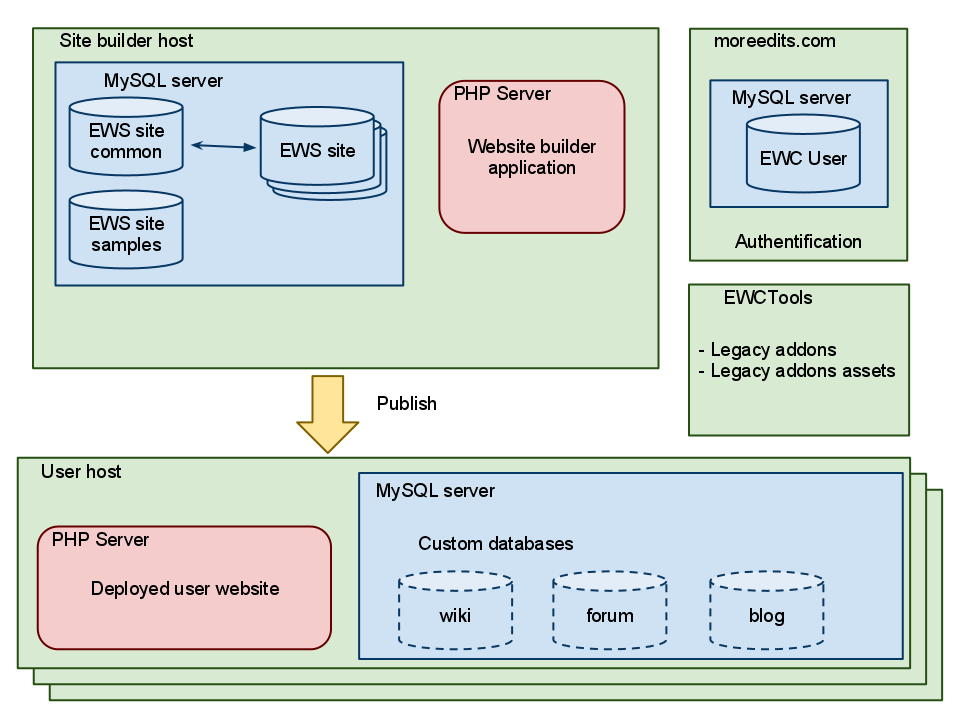
\includegraphics[width=.55\textwidth]{img/ews_archi_before.png}
\caption{Basic EWS architecture }
\label{figure:ews_archi_after}
\end{figure}


\begin{figure}[!ht]
\centering
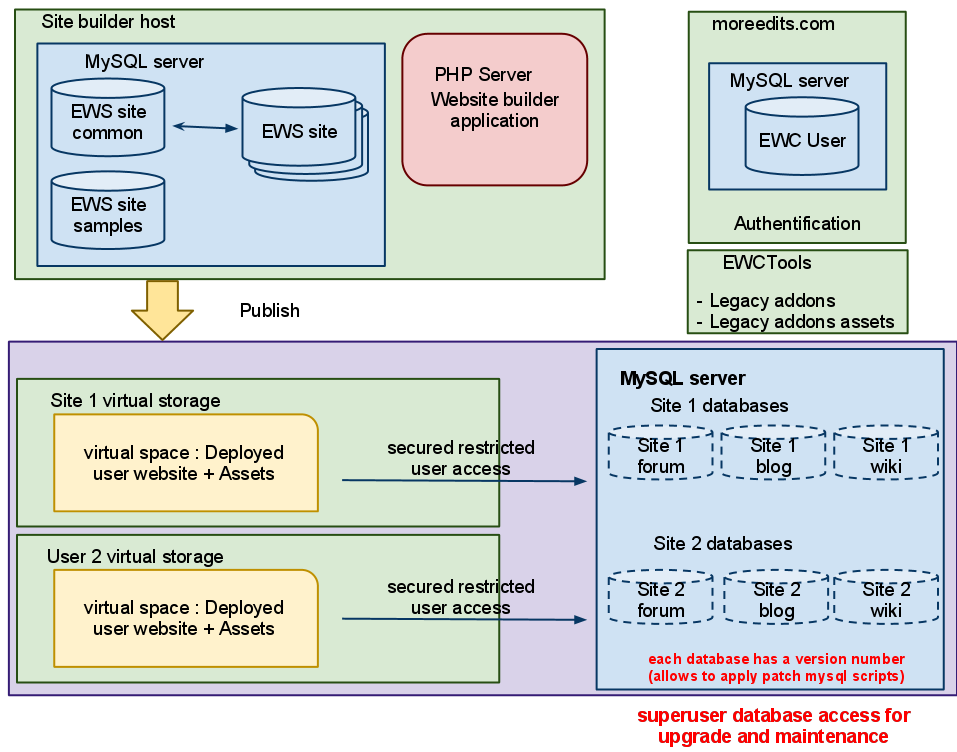
\includegraphics[width=.55\textwidth]{img/ews_archi_after.png}
\caption{EWS architecture rethink for cloud environment}
\label{figure:ews_archi_after}
\end{figure}


To allow scalability security and future cloud architecture, we decided to split the application into several databases inside the same MySQL server. Inside the same MySQL server the databases can communicate easily with each other. So it allows to decouple these databases.
\begin{itemize}
\item a database to store common data
\item a database to manage users and sites
\item one database per site 
\end{itemize}
To allow better security, at the creation of a new site database ze create a specific MySQL user for this database which have specific permissisons only on that database. It can acces common database data thru VIEWS.
% databases architecture illustration
After several meetings we decided to adopt a system that stores the informations of each pages created by the editor into a datababase.And then when the user decides he will publish the pages that are converted in plain php or html pages.

